
%(BEGIN_QUESTION)
% Copyright 2007, Tony R. Kuphaldt, released under the Creative Commons Attribution License (v 1.0)
% This means you may do almost anything with this work of mine, so long as you give me proper credit

Digital control valve positioners need a way to sense valve stem position, in order that they may control that position in accordance with the output signal sent by the process controller to the valve.  One easy way to do this is to use a {\it potentiometer} to translate stem position into a voltage that a microprocessor-based positioner can sense.  Another way is to use a {\it Hall Effect sensor}.

The Hall Effect is the generation of a (small) voltage in relative proportion to an electric current and an external magnetic field, all three being perpendicular to one another:

$$V_{Hall} = K {IB \over x}$$

$$\includegraphics[width=15.5cm]{i01700x01.eps}$$

Given a constant electric current ($I$) through the Hall Effect chip, then, the Hall voltage becomes a direct expression of the perpendicular magnetic field's intensity and direction.

\filbreak

To exploit this principle for the purpose of linear (sliding stem) valve position detection, we may place a Hall Effect chip between two magnet assemblies as such, the Hall Effect sensor being stationary and the magnet assembly attached to the valve's stem so it moves up and down with it:

$$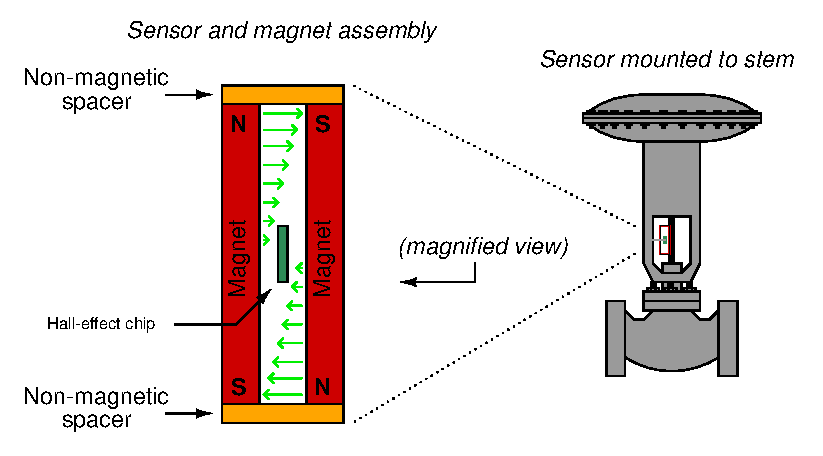
\includegraphics[width=15.5cm]{i01700x02.eps}$$

Examine this setup and then explain how the Hall Effect sensor is able to detect valve stem position.  In other words, what sort of voltage signal would you expect from the Hall Effect sensor at various stem positions?  Be as specific as you can in your answer.

\underbar{file i01700}
%(END_QUESTION)





%(BEGIN_ANSWER)

The Hall Effect sensor will output zero voltage when it is perfectly centered in the magnet assembly's length of travel (as shown in the illustration).

%(END_ANSWER)





%(BEGIN_NOTES)

The closer the sensor gets to the top of the magnet assembly, the more voltage it will generate in one direction.  The closer it gets to the bottom of the magnet assembly, the more voltage it will generate in the other direction:

$$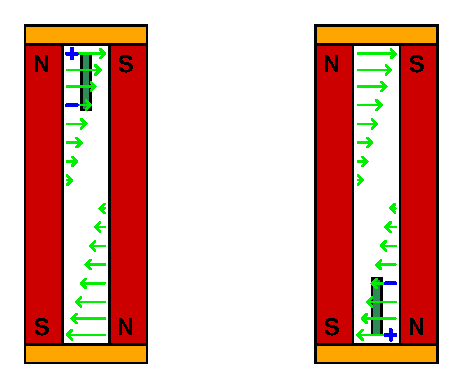
\includegraphics[width=15.5cm]{i01700x03.eps}$$

%INDEX% Electronics review: Hall Effect sensor
%INDEX% Final Control Elements, valve: positioner (electronic stem position feedback)

%(END_NOTES)


